% !TEX root = main.tex

\section{Extending SCXML}
\label{sect:extension}

\begin{figure*}
% \centering
\begin{minipage}[]{.5\textwidth}
  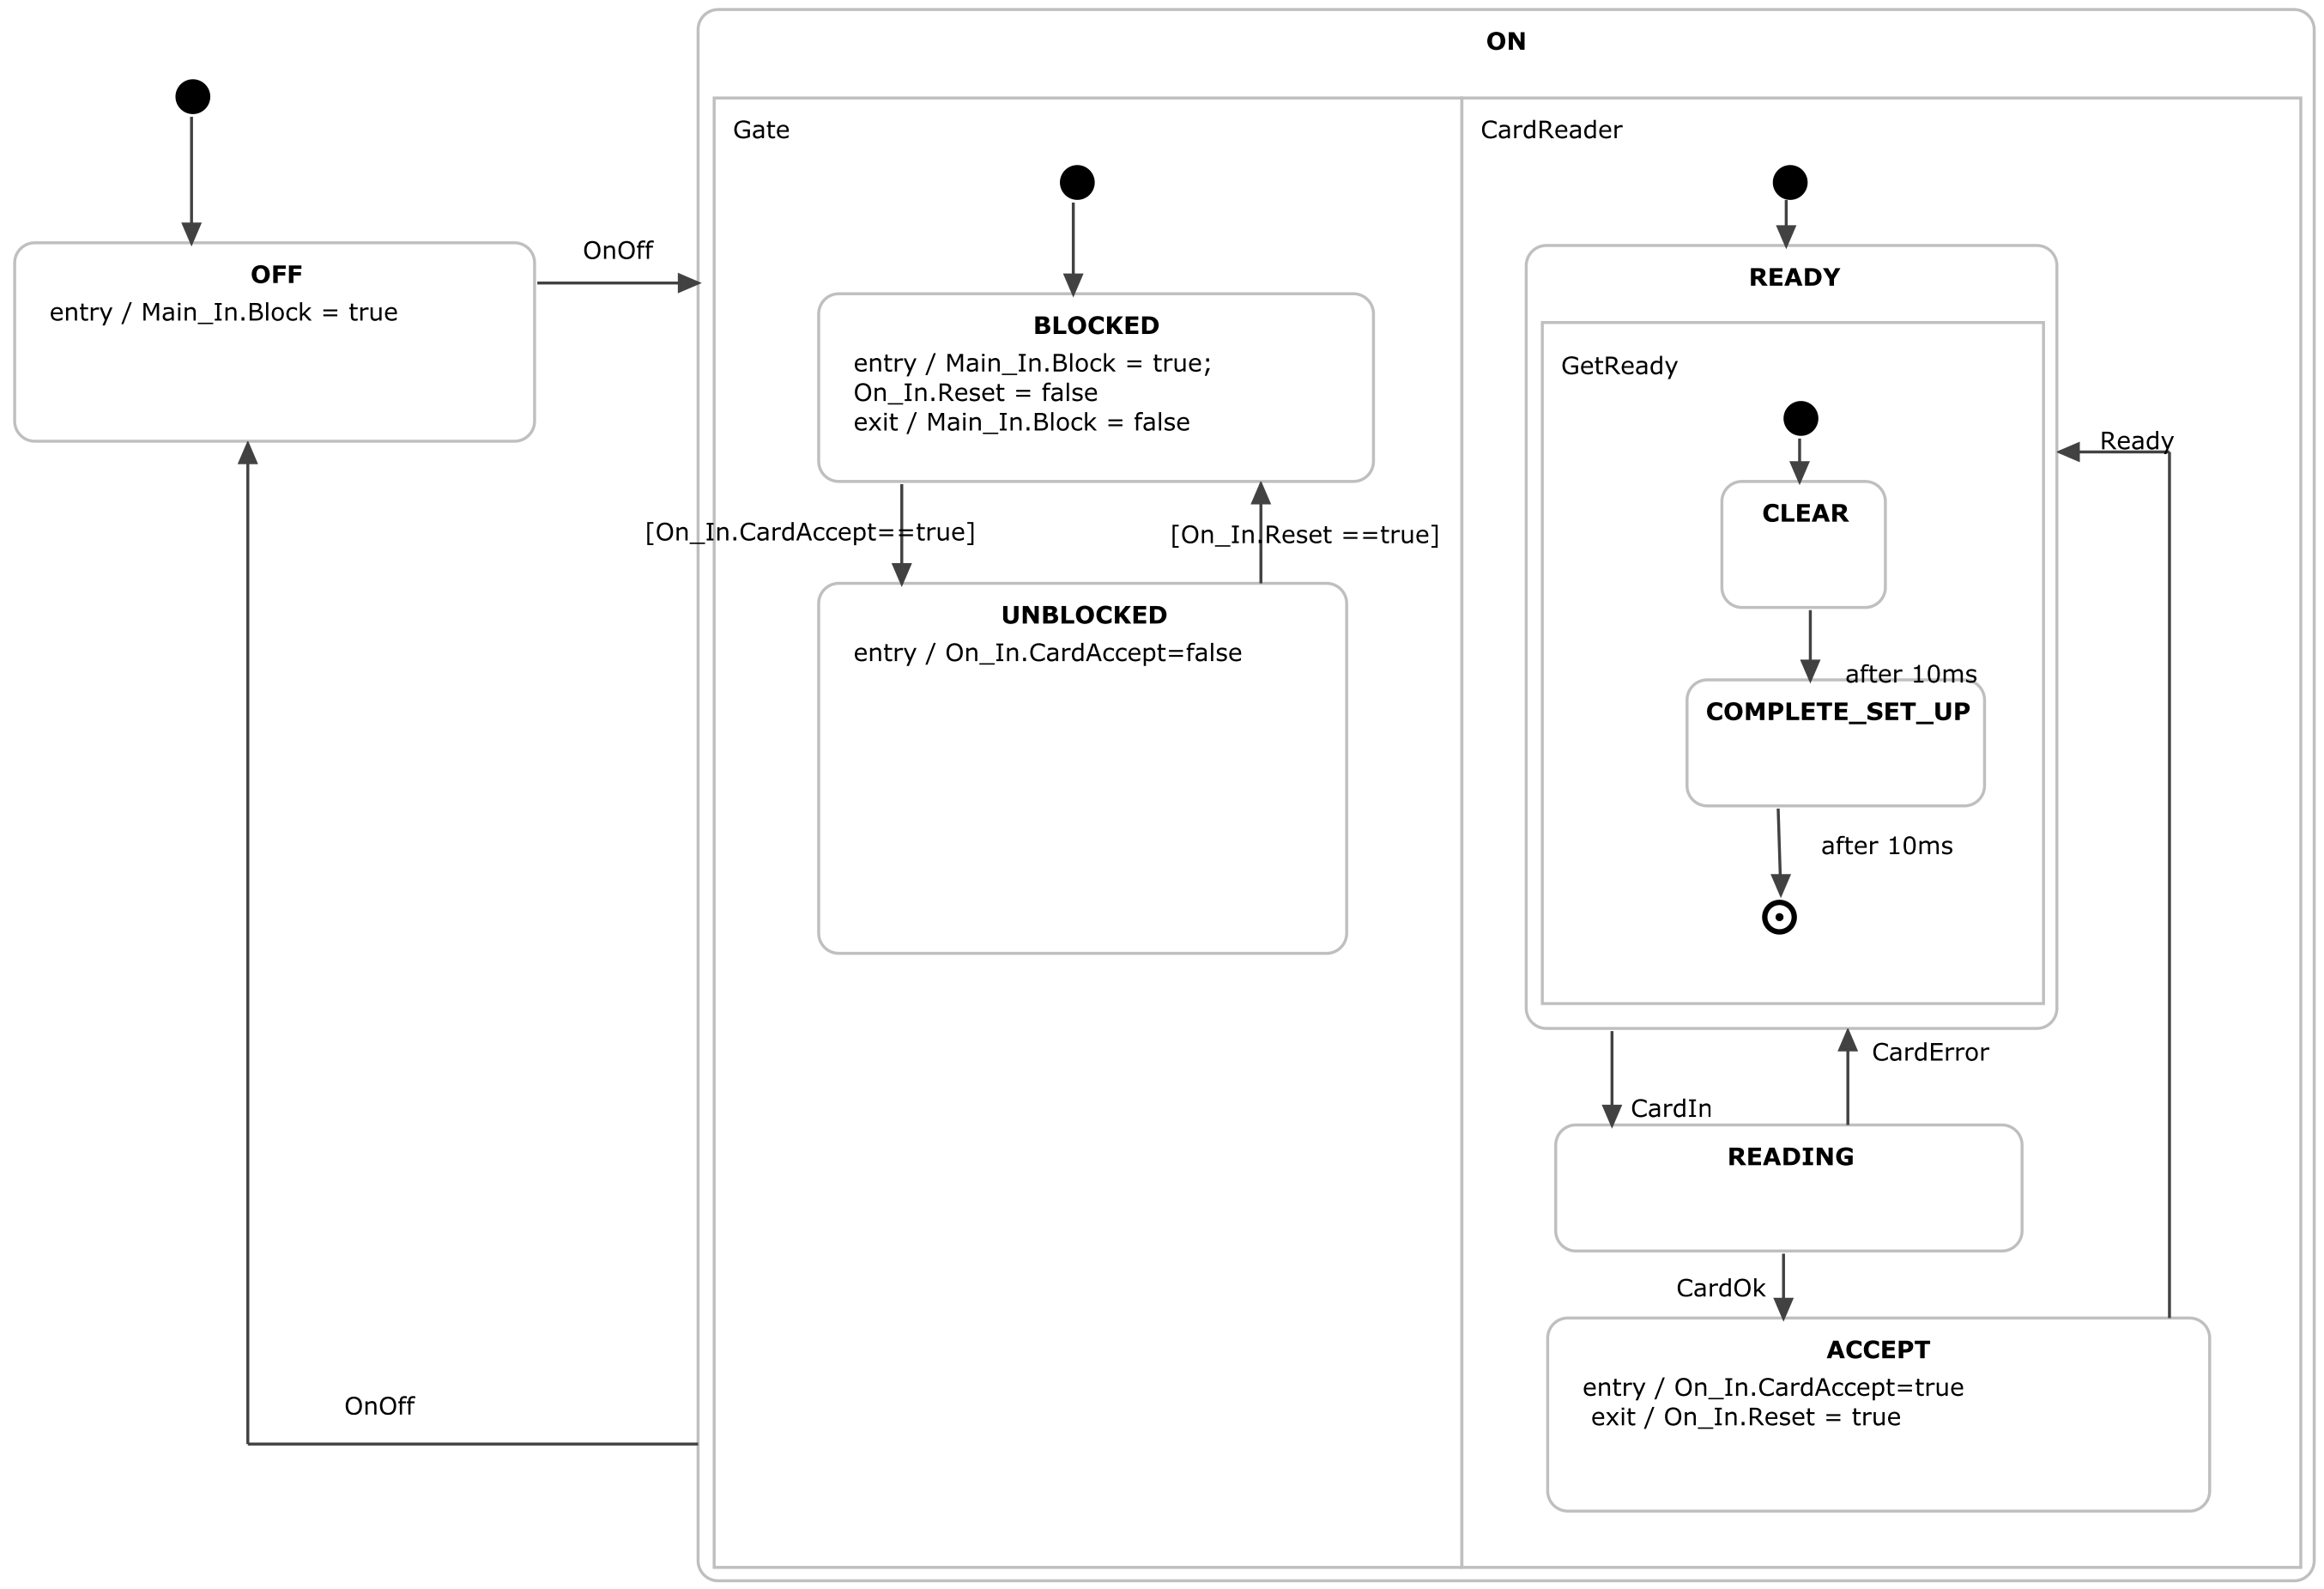
\includegraphics[width=1\textwidth]{caseStudy/TurnstileSimpleModel2.png}
  \caption{SCXML Statechart diagram}
  \label{fig:StatemachineSCXML}
\end{minipage}
\begin{minipage}[]{.5\textwidth}
  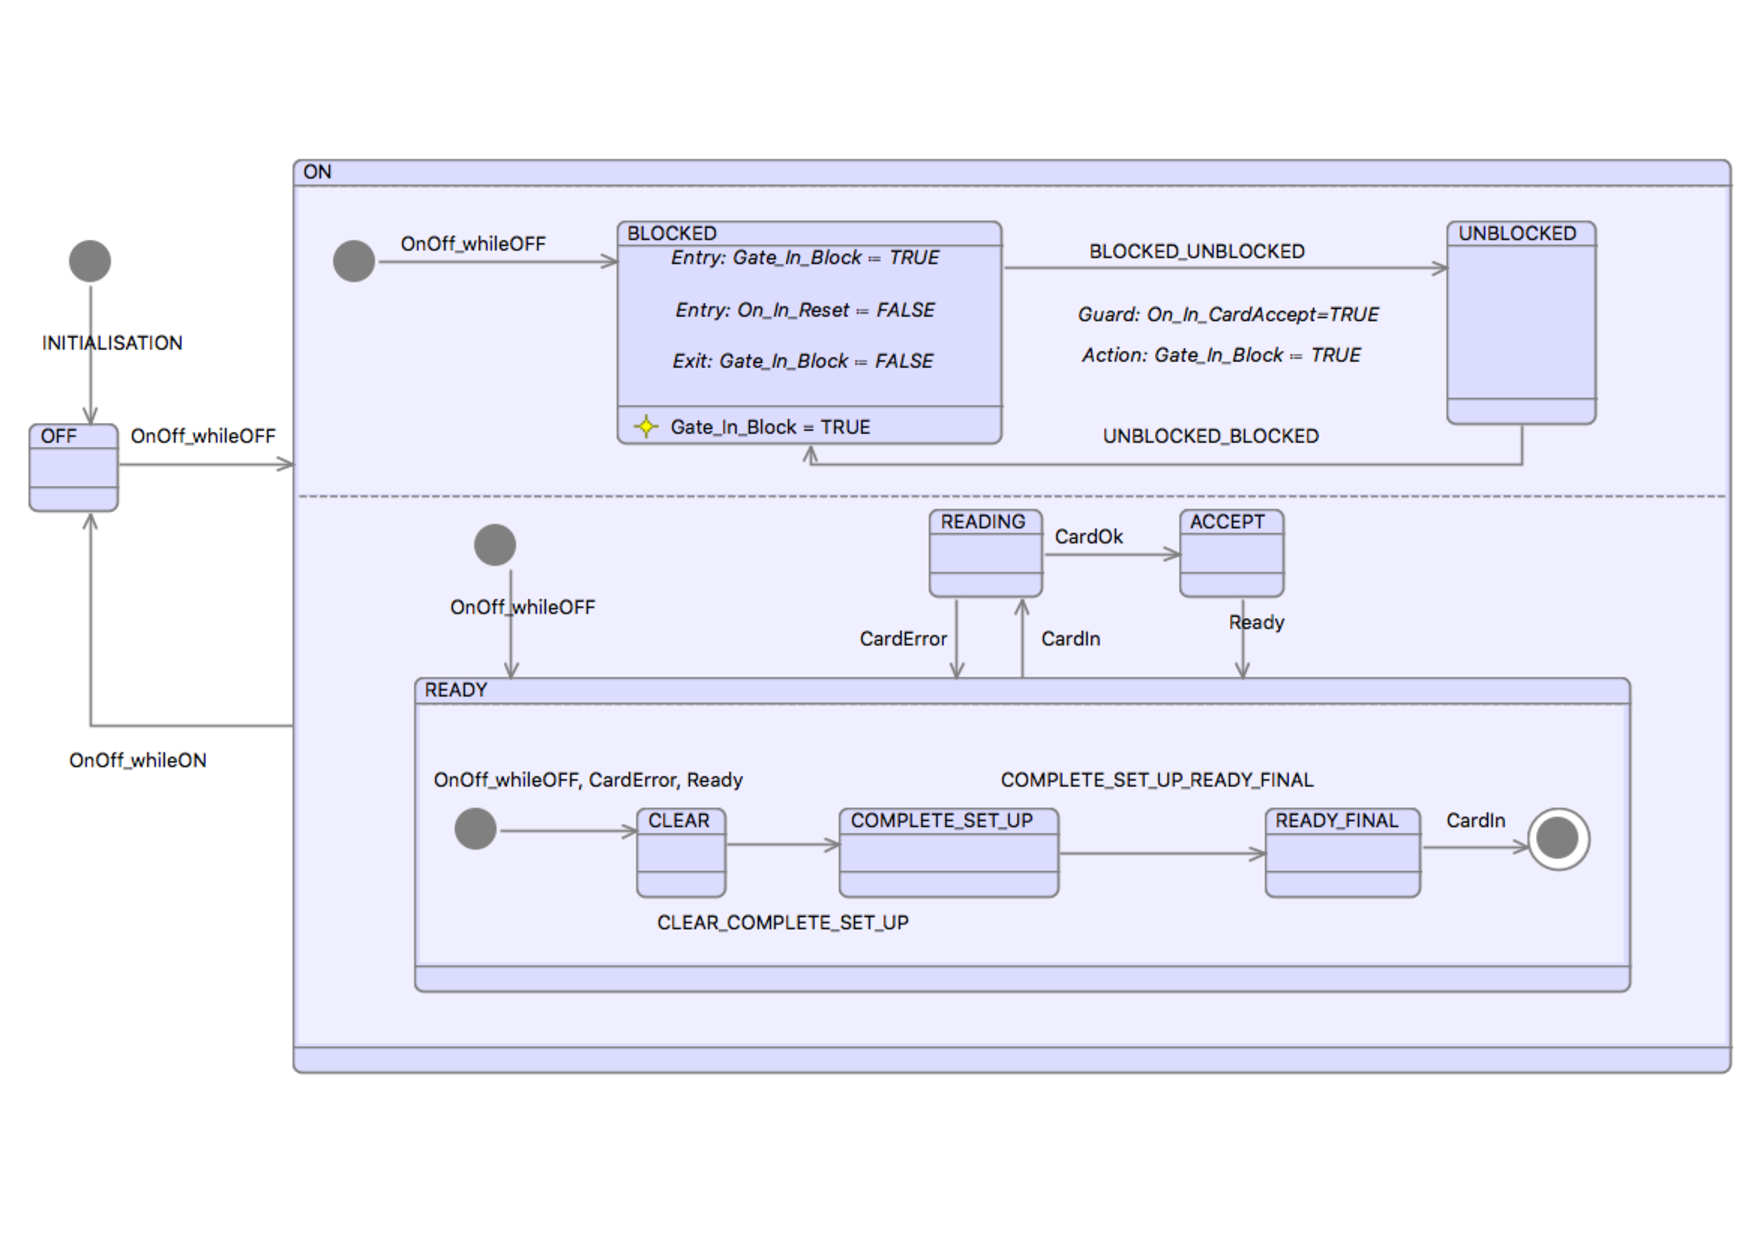
\includegraphics[width=1\textwidth]{caseStudy/TurnstileSimpleModel_iumlb}
  \caption{State-machine diagram in iUML-B at refinement level 3 (partially annotated with guards and actions)}
  \label{fig:StatemachineiUML-B}
\end{minipage}
% \caption{ and }
\end{figure*}

\fvset{frame=single,numbers=left,fontsize=\relsize{-2},numbersep=8pt}
\begin{figure}[tbp!]
  \VerbatimInput[samepage=false]{caseStudy/BlockState_Invariant.scxml}
  \caption{Part of SCXML model corresponding to figure \ref{fig:StatemachineSCXML} 
   (including iumlb extension elements explained in section \ref{sect:extension}) } 
  \label{fig:scxml}
\end{figure}

To facilitate Event-B formal verification, extensions to the SCXML 
modelling notation are necessary so that additional modelling features 
required by Event-B can be integrated with the SCXML model.
An example statechart model is shown in figure \ref{fig:StatemachineSCXML}, and a section of the corresponding SCXML syntax is shown in figure \ref{fig:scxml}. The iUML-B representation of the model is shown in figure \ref{fig:StatemachineiUML-B}. 
We use this example to illustrate different points throughout the manuscript.
The SCXML schema allows extension elements and attributes belonging 
to a different namespace to be added. 
The SCXML tooling provides fallback mechanisms so that these extensions are supported 
without the need for syntactic definition. We define a new namespace,  
\emph{iumlb} and add two new elements, \emph{iumlb:invariant} and 
\emph{iumlb:guard} as well as a 
% \emph{iumlb:guard} (Table \ref{iumlb_elements_table}) as well as a 
number of new attributes which are shown in Table \ref{iumlb_attributes_table}.
Invariants are not supported in SCXML but are needed to describe 
verifiable properties of a model. 
SCXML transitions only have a single \emph{cond} attribute whereas we need to introduce conjuncts of a transition
condition at various refinement steps. 
We also need to be able to designate some 
invariants or guards as theorems that can be derived from the preceding conjuncts. 
New attributes are introduced to support the predicate (string) and the 
derived (boolean) theorem property of invariants and guards. The concept 
of refinement is not supported in SCXML. We introduce a new integer valued 
attribute, \emph{iumlb:refinement}, which may be attached to any element of 
either namespace in order to specify the refinement level of that element. 


Figure \ref{fig:scxml} shows a state, \emph{BLOCKED}, 
containing a transition that owns an \emph{iumlb:guard}.
The guard reflects the \emph{cond} attribute of the transition 
and is introduced at refinement level 2. 
The state also owns an \emph{iumlb:invariant} with the predicate
 \emph{Gate\_In.Block == TRUE}.



% \begin{table}
% \centering
% \caption{New Elements}
% \label{iumlb_elements_table}
%   \begin{tabular}{|c|c|c|}
%   \hline
%           \multicolumn{1}{c}{Element in iumlb:} \vline
%         & \multicolumn{1}{c}{Meaning} \vline
%         & \multicolumn{1}{c}{Legal Attributes in iumlb:} 
%         \\ \hline 

%     invariant
%         & \begin{tabular}[c]{@{}c@{}} 
%               generates an invariant \\ in Event-B or iUML-B 
%           \end{tabular}     
%         & \begin{tabular}[c]{@{}c@{}}
%               % name, derived, \\ refinement,
%               % predicate, \\ comment
%               name, refinement, \\
%               predicate, derived
%           \end{tabular} 
%         \\ \hline 

%     guard 
%         & \begin{tabular}[c]{@{}c@{}} 
%               generates a guard  \\ in Event-B or iUML-B
%           \end{tabular}    
%         & \begin{tabular}[c]{@{}c@{}}
%               % name, derived, \\ refinement, 
%               % predicate, \\ comment
%               name, refinement, \\
%               predicate, derived
%           \end{tabular} 
%         \\ \hline     
% \end{tabular}%
% \end{table}

\begin{table}
\centering
\caption{SCXML Extension Attributes}
\label{iumlb_attributes_table}
  \begin{tabular}{|c|c|c|}
  \hline
      \multicolumn{1}{c}{Attribute name:} \vline
    & \multicolumn{1}{c}{Meaning} \vline
    & \multicolumn{1}{c}{Allowed Parents} 
   \\ \hline 

    label
        & \begin{tabular}[c]{@{}c@{}} 
              string used as the name of an \\
              Event-B event elaborated by \\
              the generated i-UML-B
          \end{tabular}    
        & \begin{tabular}[c]{@{}c@{}}
              scxml:transition
          \end{tabular} 
   \\ \hline 

    refinement
        & \begin{tabular}[c]{@{}c@{}} 
              non-negative integer representing \\
              the refinement level at which \\
              the parent element should \\
              be introduced
          \end{tabular}    
        & \begin{tabular}[c]{@{}c@{}}
              scxml:scxml, scxml:datamodel, \\ 
              scxml:data, scxml:state, \\
              scxml:parallel, scxml:transition, \\
              scxml:onEntry, scxml:onExit, \\
              scxml:assign, iumlb:invariant, \\
              iumlb:guard
          \end{tabular} 
   \\ \hline 

   %  iumlb:comment
   %      & \begin{tabular}[c]{@{}c@{}} 
   %            string used as a comment \\
   %            on the generated \\
   %            iUML-B element
   %        \end{tabular}    
   %      & \begin{tabular}[c]{@{}c@{}}
   %            iumlb:invariant, iumlb:guard, \\
   %            (could be added to more)
   %        \end{tabular} 
   % \\ \hline 

    type
        & \begin{tabular}[c]{@{}c@{}} 
              string used as the membership \\
              set for the Event-B variable \\
              generated from the parent \\
              data element
          \end{tabular}    
        & \begin{tabular}[c]{@{}c@{}}
              scxml:data
          \end{tabular} 
   \\ \hline 

    name
        & \begin{tabular}[c]{@{}c@{}} 
              string used for the name \\
              or label of a generated \\
              iUML-B element
          \end{tabular}    
        & \begin{tabular}[c]{@{}c@{}}
              iumlb:invariant, iumlb:guard
          \end{tabular} 
   \\ \hline 

    predicate
        & \begin{tabular}[c]{@{}c@{}} 
              string used for the predicate \\
              of a guard or invariant
          \end{tabular}    
        & \begin{tabular}[c]{@{}c@{}}
              iumlb:invariant, iumlb:guard
          \end{tabular} 
   \\ \hline 

   derived
        & \begin{tabular}[c]{@{}c@{}} 
              boolean indicating that \\
              the guard is a theorem \\
              (default to false)
          \end{tabular}    
        & \begin{tabular}[c]{@{}c@{}}
              iumlb:invariant, iumlb:guard
          \end{tabular}       
   \\ \hline 
\end{tabular}%
\end{table}

%------------------------------------------------------------------------------
